\documentclass[10pt]{article}

\usepackage{graphicx}
\usepackage{amsmath,amsfonts,amssymb}

\usepackage{hyperref}  % for urls and hyperlinks


\setlength{\textwidth}{6.2in}
\setlength{\oddsidemargin}{0.3in}
\setlength{\evensidemargin}{0in}
\setlength{\textheight}{8.9in}
\setlength{\voffset}{-1in}
\setlength{\headsep}{26pt}
\setlength{\parindent}{0pt}
\setlength{\parskip}{5pt}




% a few handy macros

\newcommand\matlab{{\sc matlab}}
\newcommand{\goto}{\rightarrow}
\newcommand{\bigo}{{\mathcal O}}
\newcommand{\half}{\frac{1}{2}}
%\newcommand\implies{\quad\Longrightarrow\quad}
\newcommand\reals{{{\rm l} \kern -.15em {\rm R} }}
\newcommand\complex{{\raisebox{.043ex}{\rule{0.07em}{1.56ex}} \hskip -.35em {\rm C}}}


% macros for matrices/vectors:

% matrix environment for vectors or matrices where elements are centered
\newenvironment{mat}{\left[\begin{array}{ccccccccccccccc}}{\end{array}\right]}
\newcommand\bcm{\begin{mat}}
\newcommand\ecm{\end{mat}}

% matrix environment for vectors or matrices where elements are right justifvied
\newenvironment{rmat}{\left[\begin{array}{rrrrrrrrrrrrr}}{\end{array}\right]}
\newcommand\brm{\begin{rmat}}
\newcommand\erm{\end{rmat}}

% for left brace and a set of choices
\newenvironment{choices}{\left\{ \begin{array}{ll}}{\end{array}\right.}
\newcommand\when{&\text{if~}}
\newcommand\otherwise{&\text{otherwise}}
% sample usage:
%  \delta_{ij} = \begin{choices} 1 \when i=j, \\ 0 \otherwise \end{choices}


% for labeling and referencing equations:
\newcommand{\eql}{\begin{equation}\label}
\newcommand{\eqn}[1]{(\ref{#1})}
% can then do
%  \eql{eqnlabel}
%  ...
%  \end{equation}
% and refer to it as equation \eqn{eqnlabel}.  


% some useful macros for finite difference methods:
\newcommand\unp{U^{n+1}}
\newcommand\unm{U^{n-1}}

% for chemical reactions:
\newcommand{\react}[1]{\stackrel{K_{#1}}{\rightarrow}}
\newcommand{\reactb}[2]{\stackrel{K_{#1}}{~\stackrel{\rightleftharpoons}
   {\scriptstyle K_{#2}}}~}

% Parts:

% set enumerate to give parts a, b, c, ...  rather than numbers 1, 2, 3...
\renewcommand{\theenumi}{\alph{enumi}}
\renewcommand{\labelenumi}{(\theenumi)}

% set second level enumerate to give parts i, ii, iii, iv, etc.
\renewcommand{\theenumii}{\roman{enumii}}
\renewcommand{\labelenumii}{(\theenumii)}

  % input some useful macros

\begin{document}

% header:
\hfill\vbox{\hbox{AMath 585}
\hbox{Homework \#2}\hbox{Due Thursday, January 23, 2019}}

\vskip 5pt

Homework is due to Canvas by 11:00pm PDT on the due date.

To submit, see
\url{https://canvas.uw.edu/courses/1352870/assignments/5223966}



%--------------------------------------------------------------------------
\vskip 1cm
\hrule
{\bf Problem 1.}

Consider a ``rigid'' beam of length $L$
that is supported at both ends and sags by a very
small amount in the center due to gravity acting on the mass.  The small
deflection can be modeled by the Euler-Bernoulli 
beam equation described for example at\\
\url{https://en.wikipedia.org/wiki/Euler-Bernoulli\_beam\_theory}, \\
which in the simplest case where the beam has constant
cross-sectional area and is made of a uniform material takes the simple form
\[
u''''(x) = \gamma, \qquad \text{for~} 0\leq x \leq L,
\]
where $\gamma$ is a constant depending on the material properties.   
If both ends are embedded in walls that hold their position constant 
(at $u=0$, say) and also hold them horizontal at the ends, then the boundary
conditions are
\[
u(0) = u'(0) = 0, \qquad u(L) = u'(L) = 0.
\]
The deflection then looks something like this (with a greatly exagerated
vertical scale):

\hfil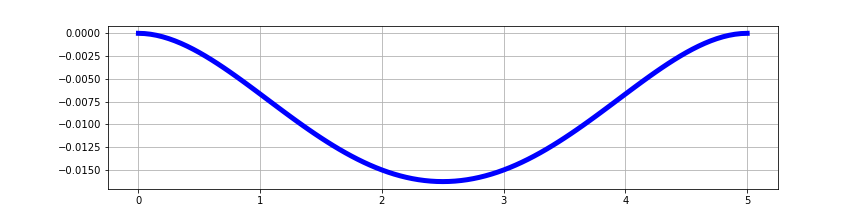
\includegraphics[width=6.0in]{beam.png}\hfil

(a) The exact solution to this problem is easy to compute as a quartic
function that satisfies the four boundary conditions.  Compute this for
$L=5$ and $\gamma = 0.01$, and confirm that it looks like the figure above.

(b) Write a computer program to solve this problem.  Use the second-order
accurate formula for the fourth derivative that you derived in Homework 1,
together with formulas for boundary conditions that preserve the second
order accuracy.  There is more than one way to do this that would be correct.

Test your program for a series of grids and produce a
log-log plot to verify the expected accuracy.


% uncomment the next two lines if you want to insert solution...
%\vskip 1cm
%{\bf Solution:}

% insert your solution here!

%--------------------------------------------------------------------------
\vskip 1cm

\hrule
{\bf Problem 2.}  
The problem above doesn't fully test whether the boundary conditions are
implemented properly since the values specified are all zero.

To test your code a bit more, adapt it to solve the problem $u''''(x) = f(x)$
on the interval $0 \leq x \leq 1$ with the function $f(x)$ and boundary
conditions on $u(0),~u'(0),~u(1),$ and $u'(1)$ chosen so that the true
solution is $u(x) = 2 + 3x + x^5$.  (This is the method of manufactured
solutions as discussed in the notebook {\tt BVP1.ipynb}.)

% uncomment the next two lines if you want to insert solution...
%\vskip 1cm
%{\bf Solution:}

% insert your solution here!

%--------------------------------------------------------------------------
\vskip 1cm
\newpage

\hrule
{\bf Problem 3.}  The notebook {\tt BVP\_stability.ipynb} (visible as a
rendered webpage
\href{https://rjleveque.github.io/amath585w2020/notebooks/html/BVP\_stability.html}{here})
shows plots of the columns of $A^{-1}$ that correspond to the discussion of
Section 2.11 and Figure 2.1 in the book.  Also shown are similar plots for
the case of Neumann boundary conditions at the left boundary.  

The plot below shows the columns in the simpler case where the matrix 
from (2.54) is used for the Neumann boundary condition, for the case $m=5$. 


\hfil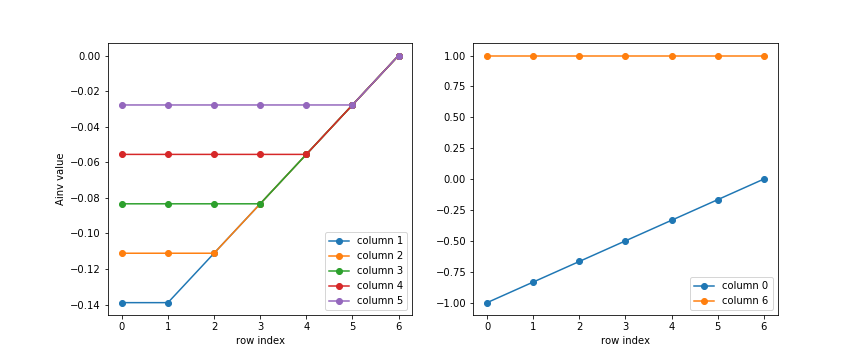
\includegraphics[width=6.0in]{NeumannAinv.png}\hfil

(a) Explain why each of these has the form it does, and give 
a closed form expression for all elements of $A^{-1}$ in the general case
with $m$ interior points (similar to (2.46) for the Dirichlet case).

(b) Using this formula, obtain an upper bound on $\|A^{-1}\|_\infty$
that is independent of $h$ in order to prove stability of this method.

(c) Determine the Green's function for the problem with the Neumann condition
at the left boundary, i.e. the function $G(x; \bar x)$ that solves
\[
u''(x) = \delta(x-\bar x), \qquad \text{for~} 0\leq x \leq 1,
\]
with boundary conditions
\[
u'(0) = 0, u(1) = 0.
\]

% uncomment the next two lines if you want to insert solution...
%\vskip 1cm
%{\bf Solution:}

% insert your solution here!



%--------------------------------------------------------------------------

\end{document}
